\documentclass[10pt,a4paper]{article}
\usepackage[utf8]{inputenc}
\usepackage{amsmath}
\usepackage{amsfonts}
\usepackage{amssymb}
\usepackage{graphicx}
\author{José Jácome}
\title{Resolución de EDP y EDO mediante Matlab}
\begin{document}
\setlength{\unitlength}{1 cm} %Especificar unidad de trabajo
\thispagestyle{empty}
\begin{picture}(18,4)
\put(-3,0){
\includegraphics[scale=0.5]{ESPE.png}}
\put(9.5,0){
\includegraphics[scale=0.25]{Mecatronica.png}}
\end{picture}
\\
\\
\begin{center}
\textbf{{\Huge UNIVERSIDAD DE LAS FUERZAS ARMADAS}\\[0.5cm]
{\LARGE ESPE EXTENSIÓN LATACUNGA}}\\[1.25cm]
{\Large MATEMÁTICA SUPERIOR}\\[2.3cm]
{\LARGE \textbf{EDO y EDP con MATLAB}}\\[3.5cm]
{\large Jácome José}\\[2cm]
IV MECATRÓNICA "A"\\[1cm]
Latacunga-Ecuador - \today
\end{center}
\begin{center}
\section{Resolución de Ecuaciones Diferenciales Parciales con Matlab}
\end{center}
\subsection{Comando pdepe} 
El comando \textit{pdepe} se utiliza para resolver 	Ecuaciones Diferenciales Parciales con condiciones iniciales para ecuaciones de tipo parabólico y elíptico\\
Esta permite resolver EDP o sistemas de EDPs de una variable especial x y una variable temporal t. La forma normal de las EDPs, 
\begin{verbatim}
u = pdepe(m,@pdefun,@icfun, @bcfun,x,t)
\end{verbatim}
\subsection{Forma General de las EDP para llevar a Matlab} 
La forma normal que se pueden resolver es de la forma:\\
$c (x,t,u, \dfrac{\partial u}{\partial x}) \dfrac{\partial u}{\partial x} = \dfrac{1}{x^n} \dfrac{\partial}{\partial x} [x^m f(x,t,u,\dfrac{\partial u}{\partial x})] + s(x,t,u, \dfrac{\partial u}{\partial x})$\\
El Coeficiente c que multiplica la derivada con respecto a $t$ es una matriz diagonal que se especifica como vector. La variable especial para 	reescalarse es tener: $0 < x < 1$.\\
El Parámetro m esta asociado a la geometría del problema: m = 0,1,2 corresponde a x como la coordenada radial en coordenadas cartesianas, cilíndricas o esféricas respectivamente. \\
Los terminos $f,s$ se llaman flujo y fuente respectivamente.
\subsection{Condiciones de Frontera}
La condición de frontera en los extremos $x \in [0,1]$ se especifican en la forma:\\
$p(x,t,u) + q(x,t) f(x,t,u,\dfrac{\partial u}{\partial x})$\\
donde $x= a,b$. Es necesario especificar loas componentes de $p = (pl, pr)$ y de $q = (ql,qr)$ como funciones de t y de los valores de u en los extremos $(ul,ur)$ en el caso de p. Note que las condiciones de frontera se especifican mediante el flujo de la derivada parcial $\dfrac{\partial u}{\partial x}$
\subsection{Condiciones Iniciales}
Se especifican en la forma de una función de x\\
$u = icfun(x)$
\subsection{Llamada principal para resolver una EDP}
\begin{verbatim}
u = pdepe(m,@pdefun,@icfun, @bcfun,x,t)
\end{verbatim}
Sean $nx = length(x)$ , $nt = lenght(t)$ las longitudes de las mallas $x$ y $t$ respectivamente, $np$ es el numero de ecuaciones diferenciales, entonces:
\begin{verbatim}
a = x(1) < x(2) < ... <x(end) = b
0 = t(1) < t(2) < ... < t(end)
\end{verbatim}
La solución $u$ es un arreglo multidimensional de tamaño $nt * nx * np$ ; con $nx \geq 3$, por ejemplo $u(j,k,i)$ es la solución aproximada de la componente $i$en el punto $(t(j),x(k))$.
Nótese que los índices $j,k$ corresponden al orden de las variables $(t,x)$.\\
Las funciones en el argumento de pdepe siguen la sintaxis:
\subsection{Flujo} 
\begin{verbatim}
[c,f,s] = pdefun(x,t,u,dudx)
\end{verbatim}
donde $x, t$ son escalares, $u, dudx$ son vectores de dimensión np. La función regresa
vectores c,f,s de de dimensión np correspondientes a la matriz diagonal $c(x,t,u,\dfrac{\partial u}{\partial x} / )$,flujo $f(x,t,u ,\dfrac{\partial u}{\partial x} )$ y fuente $s(x,t,u , \dfrac{\partial u}{\partial x} )$. Por cada entrada del vector c nulo, la ecuación correspondiente es de tipo elíptica pero debe haber al menos una ecuación parabólica.

\subsection{Condiciones de frontera} 
\begin{verbatim}
[pl,ql,pr,qr] = bcfun(xl,ul,xr,ur,t)
\end{verbatim}
donde $pl, ql$ son vectores columna de dimensión np correspondientes a la función $p(a,t,u)$ y a la matriz diagonal $q(a,t,u,\dfrac{\partial u}{\partial x})$. Note que sólo p puede depender de u. Análogamente $pr, qr$ son vectores columna de dimensión
np correspondientes a la función $p(a,t,u)$ y a la matriz diagonal $q(b,t,u ,\dfrac{\partial u}{\partial x})$
\subsection{Condición inicial}
\begin{verbatim}
u = icfun(x)
\end{verbatim}
donde x es un escalar, u es un vector de dimensión np. 
\subsection{Evaluación de la solución en puntos específicos de x} 
\begin{verbatim}
ui = u(:,:,i)
\end{verbatim}
aproxima la i-ésmima componente de la solución en la malla tempo-espacial (t,x).\\
Para evaluar la solución y su derivada en puntos de la malla  $xout$ distintos de la malla x se usa el comando.
\begin{verbatim}
[uout,duoutdx] = pdeval(m,x,ui,xout)
\end{verbatim}
la salida son vectores $uout,duoutdx$ contienen las aproximaciones en la malla $xcout$.\\
Observe que se evalúa la derivada y no el flujo. 
\begin{verbatim}
Manejo de discontinuidades
\end{verbatim} 
Se permiten discontinuidades de cos en x siempre que se incluyan en la malla x, pero el
flujo deberá ser continuo. Es conveniente usar una malla más fina cerca de los puntos de
discontinuidad, pero para m =2 (coordenadas esféricas) esto no es necesario. \\
\subsection{Codigo de Matlab}
\begin{verbatim}
%Resolucion de una EDP por Matlab
function pdex1
% 20 puntos de malla especial, 5 temporal
m = 0;
x = linspace(0,1,20);
t = linspace(0,2,5);
%Llamada a la rutina principal
sol = pdepe(m,@pdex1pde,@pdex1ic,@pdex1bc,x,t);
%Primera componente
u=sol(:,:,1);
%Grafico de superficie
figure;
surf(x,t,u);
title('Solución numérica con 20 puntos de malla.');
xlabel('Distancia x');
ylabel('Tiempo t');
figure;
surf(x,t,exp(-t)'*sin(pi*x));
title('Solución exacta con 20 puntos de malla. ');
xlabel('Distance x');
ylabel('Time t');
figure;
plot(x,u(end,:), 'o',x,exp(-t(end))*sin(pi*x));
title('Soluciones en t = 2. ');
legend('Numerica, 20 puntos de malla', 'Analitica',0);
xlabel('Distancia x'); ylabel('u(x,2)');
% Especificacion de la EDP
function [c,f,s] = pdex1pde(x,t,u,DuDx)
c = pi^2;
f = DuDx;
s = 0;
% Especificación de la condición inicial
function u0 = pdex1ic(x)
u0 = sin(pi*x);
% Especificación de condiciones de frontera
function [pl,ql,pr,qr] = pdex1bc(xl,ul,xr,ur,t)
pl = ul;
ql = 0;
pr = pi * exp(-t);
qr = 1; 

\end{verbatim}
\subsection{Capturas de Pantalla}
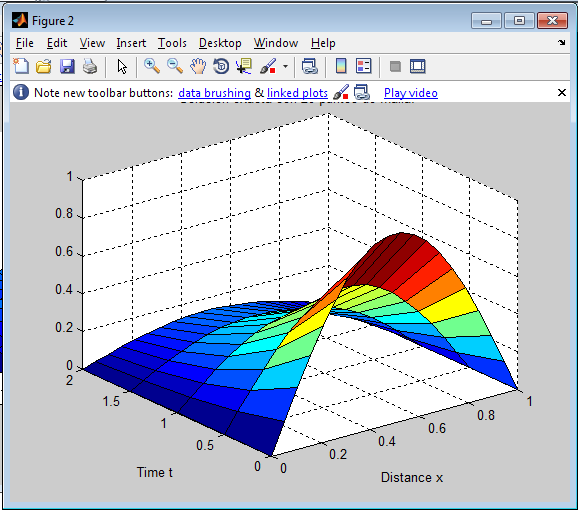
\includegraphics[scale=0.5]{Grafica1.png}\\
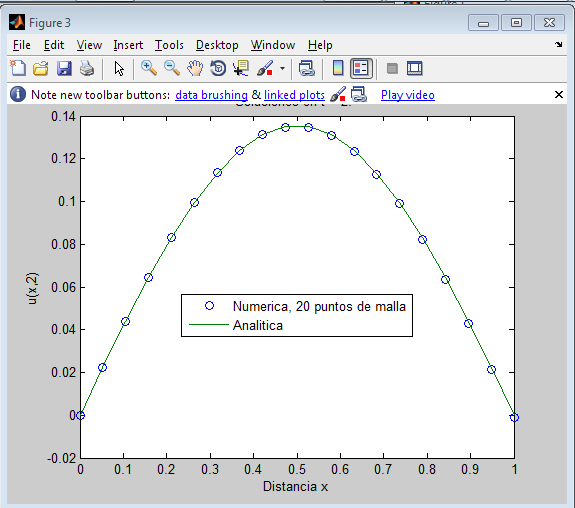
\includegraphics[scale=0.5]{Grafica2.png}
\end{document}